\section{One Way ANOVA Diagnostics}
\item The \texttt{R} code and graphical procedures, below and on the following page, are relevant to checking whether the underlying assumptions are met for an ANOVA model.
\begin{itemize}
	\item[(i.)] (2 marks) State two testable assumptions required for ANOVA procedures? (You may refer to the code output below.)
	\item[(ii.)] (2 marks)  Assess the validity of these assumptions for an ANOVA model based on the following code outputs.
	
\end{itemize}
{
	\normalsize
	\begin{framed}
		\begin{verbatim}
		> #Shapiro-Wilk normality test
		> shapiro.test(resid(model))
		
		Shapiro-Wilk normality test
		
		data:  resid(model)
		W = 0.96108, p-value = 0.4604
		
		\end{verbatim}
	\end{framed}
	\begin{framed}
		\begin{verbatim}
		> bartlett.test(investigator~group)
		
		Bartlett test of homogeneity of variances
		
		data:  investigator by group
		Bartlett's K-squared = 7.1354, df = 3, p-value = 0.0677
		
		\end{verbatim}
	\end{framed}
}



\end{itemize}


% \begin{center}
% 	\includegraphics[scale=0.59]{image/ExamQ5boxplot}
% \end{center}
% \newpage
% %qqnorm(resid(Model),pch=18,col="red",font.lab=2,font.axis=2)
% %qqline(resid(Model))
% \begin{center}
% 	\includegraphics[scale=0.55]{image/ExamQ5qqplot}
% \end{center}
% \begin{center}
% 	\includegraphics[scale=0.55]{image/ExamQ5resid}
% \end{center}



%\subsubsection*{Question 4 Part B (10 Marks)}
%
%
%
%
%The \texttt{R} code and graphical procedures, below and on the following page, are relevant to checking whether the underlying assumptions are met for the ANOVA model in part (b).
%\begin{itemize}
%	\item[i.] (3 marks) What are the assumptions underlying ANOVA?
%	\item[ii.] (4 marks)  Assess the validity of these assumptions for the ANOVA model in part(b).
%	
%\end{itemize}
%\begin{framed}
%	\begin{verbatim}
%	Shapiro-Wilk normality test
%	
%	data:  Residuals
%	W = 0.9719, p-value = 0.3819
%	\end{verbatim}
%\end{framed}
%\begin{framed}
%	\begin{verbatim}
%	Bartlett test of homogeneity of variances
%	
%	data:  Experiment
%	Bartlett's K-squared = 105.9585, df = 1, p-value < 2.2e-16
%	\end{verbatim}
%\end{framed}
%\begin{center}
%	\includegraphics[scale=0.59]{images/ExamQ5boxplot}
%\end{center}
%\newpage
%%qqnorm(resid(Model),pch=18,col="red",font.lab=2,font.axis=2)
%%qqline(resid(Model))
%\begin{center}
%	\includegraphics[scale=0.55]{images/ExamQ5qqplot}
%\end{center}
%\begin{center}
%	\includegraphics[scale=0.55]{images/ExamQ5resid}
%\end{center}
%-----------------------------------------------------------------%


%====================================================================== %
\newpage

\item Four investigators, A, B, C and D, performed six determination of nitrate in water using the same procedure. The results in $\mu$M were:

% Investigator 1 Investigator 2 Investigator 3

\begin{center}
	\begin{tabular}{|c|c|c|c|} \hline
		A  &  B   & C &D\\ \hline \hline
		6.7 & 6.3 & 6.8 & 6.9\\ \hline
		6.8 & 6.2 & 6.9 & 7.1\\ \hline
		6.5 & 6.1 & 7.1 &6.3 \\ \hline
		6.8 & 6.3 & 6.9 &6.2\\ \hline
		6.9 & 6.5 & 7.2 & 6.1\\ \hline
		7.1 & 6.4 & 7.1 & 6.4\\ \hline
	\end{tabular} 
\end{center}



\noindent We are also given the summmary statistics for each of the three investigators, as well as for the samples combined.
\begin{center}
	\begin{tabular}{|c|c|c|}
		\hline  & Sample Mean & Sample Variance \\ 
		\hline A & 6.8 & 0.040 \\ 
		\hline B & 6.3 & 0.020 \\ 
		\hline C & 7 & 0.024 \\ 
		\hline D & 6.5 &  0.164\\
		\hline Overall & 6.65 & 0.1295 \\ 
		\hline 
	\end{tabular} 
\end{center}
\noindent An analysis of variance procedure is used to determine if there is a significant difference between the mean of the determinations made by the three investigators.

% The following output is obtained in R and presented below.

%investigator <- c(6.7, 6.8, 6.5, 6.8, 6.9, 7.1, 6.3, 6.2, 6.1, 6.3, 6.5, 6.4, 
%6.8, 6.9, 7.1, 6.9, 7.2, 7.1)
%A <- investigator[1:6]
%B <- investigator[7:12]
%C <- investigator[13:18]
%
%
%
%group <- factor(rep(1:3,each=6))
%
%aov(investigator~group)
%
%Analysis of Variance Table
%
%Response: investigator

%Df SumSq MeanSq Fvalue Pr(>F)
%
%group ? 1.42333 ? ? 3.133e-05
%
%Residuals 15 ? ?
%
%Total ? 1.9
\smallskip

\noindent The following questions will result in the completion of the ANOVA Table on the next page. The $p-$value is already provided.
\begin{itemize}
	\item[(i.)](3 Marks) Compute the Between Groups Sum of Squares. (Show your workings.)
	\item[(ii.)](3 Marks) Compute the Within Groups Sum of Squares.(Show your workings.)
	\item[(iii.)](2 Marks) Compute the Total Sum of Squares. (Show your workings).
	\item[(iv.)] (1 Mark) State the degrees of freedom for the ANOVA Tables
	\item[(v.)] (1 Mark) Compute the Mean Square values.
	\item[(vi.)] (1 Marks) Compute the test Statistic for this procedure (i.e. the F-value.)
	\item[(vii.)] (3 Marks) This analysis is used to assess if there is any difference between the mean determinations made by the three investigators. What is your conclusion? Clearly state the null and alternative hypothesis.
\end{itemize}
%================================================================================ %
\begin{center}
	\begin{tabular}{|c||c|c|c|c|c|}
		\hline Source & DF & SS & MS & F & p-value \\ \hline 
		\hline Between & \phantom{mak} ? \phantom{mak}  & \phantom{mak} ? \phantom{mak}  & \phantom{mak} ? \phantom{mak}  & \phantom{mak} ? \phantom{mak}  &  $0.000454$ \\ 
		\hline Within &  ? & ? & \phantom{mak} ? \phantom{mak}  &  &  \\ 
		\hline \hline Total & ? & ? &  &  &  \\ 
		\hline 
	\end{tabular}
\end{center} 



\item[(d)]

%% \subsection*{Part C Battery - Partial Completion ANOVA (MA4605)}

An engineer is designing a battery for use in a device that will be subjected to some extreme variations in temperature. 

The only design parameter that he can select at this point is the plate material for the battery, and he has three possible choices. 
When the device is manufactured and is shipped to the field, the engineer has no control over the temperature extremes that the device will encounter, and he knows from experience  that temperature will probably affect the effective battery life. 

However, temperature can be controlled in the product development laboratory for the purposes of a test.  The engineer decides to test all three place materials at three temperature levels – 15, 70, and 125 degrees. 

Four batteries are tested at each combination of plate material and temperature, and all 36 tests are run in random order.


The following partial ANOVA table resulted:

Analysis of Variance for Battery Life Data
%----------------------------------------------
\begin{center}
	\begin{tabular}{|l|c|c|c|}\hline
		Source of & Sum of &\phantom{mak} Degrees of \phantom{mak}& Mean \\
		
		Variation & Squares & Freedom  & Square\\
		
		Material types & 2&  10,683.72 & \phantom{mak} 5,341.86\phantom{mak} \\
		
		Temperature & 2& 39,118.72 & 19,559.36\\
		
		Interaction & 4& 9,613.78 & 2,403.44\\
		
		Error &\phantom{mak} 27\phantom{mak}& 18,230.75 & 675.21\\
		
		Total &35&77,646.97 & \\\hline
	\end{tabular} 
\end{center}
% ----------------------------------------------
\begin{itemize}
	\item[(i.)] Carry out appropriate tests stating clearly the null hypotheses and conclusions. 
	
	\item[(ii.)] Would the engineer be satisfied with his design of the experiment? Explain your answer. 
\end{itemize}


\newpage



\item[(e)] The \texttt{R} code and graphical procedures, below and on the following page, are relevant to checking whether the underlying assumptions are met for the ANOVA model in part (b).
\begin{itemize}
	\item[(i.)] (3 marks) What are the assumptions underlying ANOVA?
	\item[(ii.)] (4 marks)  Assess the validity of these assumptions for the ANOVA model in Part B.
	
\end{itemize}
\begin{framed}
	\begin{verbatim}
	Shapiro-Wilk normality test
	
	data:  Residuals
	W = 0.9719, p-value = 0.3819
	\end{verbatim}
\end{framed}
\begin{framed}
	\begin{verbatim}
	Bartlett test of homogeneity of variances
	
	data:  Experiment
	Bartlett's K-squared = 105.9585, df = 1, p-value < 2.2e-16
	\end{verbatim}
\end{framed}
\begin{center}
	\includegraphics[scale=0.59]{images/ExamQ5boxplot}
\end{center}
\newpage
%qqnorm(resid(Model),pch=18,col="red",font.lab=2,font.axis=2)
%qqline(resid(Model))
\begin{center}
	\includegraphics[scale=0.55]{images/ExamQ5qqplot}
\end{center}
\begin{center}
	\includegraphics[scale=0.55]{images/ExamQ5resid}
\end{center}%
%====================================================================== %


%
%
%\begin{itemize}
%	\item[(i)](3 Marks) Compute the Between Groups Sum of Squares, \textit{Show your workings}
%	\item[(ii)](3 Marks) Compute the Within Groups Sum of Squares, \textit{Show your workings}
%	\item[(iii)](2 Marks) Compute the Total Sum of Squares,\textit{ show your workings}
%	\item[(iv)] (2 Marks) Degrees of Fredom columns
%	\item[(v)] (1 Marks) Mean Square
%	\item[(vi)] (1 Marks) F test Statistics
%\end{itemize}
%\begin{tabular}{|c|c|c|c|c|c|}
%	\hline Source & DF & SS & MS & F & p-value \\ 
%	\hline Between &  &  &  &  &  \\ 
%	\hline Within &  &  &  &  &  \\ 
%	\hline Total &  &  &  &  &  \\ 
%	\hline 
%\end{tabular} 
%\begin{framed}
%	\begin{verbatim}
%	> bartlett.test(y~group)
%	
%	Bartlett test of homogeneity of variances
%	
%	data:  y by group
%	Bartlett's K-squared = 7.9063, df = 2, p-value = 0.01919
%	
%	\end{verbatim}
%\end{framed}
